%----------------------------------------------------------------------------------------
%	PACKAGES AND OTHER DOCUMENT CONFIGURATIONS
%----------------------------------------------------------------------------------------

\documentclass[10pt,a4paper,twoside]{article} % 10pt font size, A4 paper and two-sided margins

\PassOptionsToPackage{dvipsnames}{xcolor}

\usepackage[french]{babel}

\usepackage[top=2cm,bottom=2cm,left=1.9cm,right=1.9cm,columnsep=30pt]{geometry} % Document margins and spacings

\usepackage[utf8]{inputenc} % Required for inputting international characters
\usepackage[T1]{fontenc} % Output font encoding for international characters
\usepackage{palatino} % Use the Palatino font

\usepackage{microtype} % Improves spacing

\usepackage{multicol} % Required for splitting text into multiple columns

\usepackage[bf,sf,center]{titlesec} % Required for modifying section titles - bold, sans-serif, centered

\usepackage{sectsty}                % Secion titles

\usepackage{gensymb}                % Symboles

\usepackage{tikz}
\usepackage{eso-pic}               % put things into background 
\usepackage{rotating}               % Text rotation 
\usepackage{ifthen}                 % If then package
\usepackage{graphicx}               

\usepackage{xcolor}    				% Color package
\usepackage{bclogo}                 % To get \bcloupe

\usepackage{xstring}
\usepackage{lettrine}               % First letter as a capital letter

\usepackage[hidelinks]{hyperref}    % For first letter link

\usepackage{fancyhdr}               % Required for modifying headers and footers

\usepackage{extramarks}             % For header

\usepackage[pages=all]{background}  % Background

\usepackage{blindtext}              % For links

\setlength{\headheight}{13pt}

% ------------------------------------------------------------
% Présence des lettres dans le dictionnaire
% ------------------------------------------------------------

\newif\ifletterA \letterAfalse
\newif\ifletterB \letterBfalse
\newif\ifletterC \letterCfalse
\newif\ifletterD \letterDfalse
\newif\ifletterE \letterEfalse
\newif\ifletterF \letterFfalse
\newif\ifletterG \letterGfalse
\newif\ifletterH \letterHfalse
\newif\ifletterI \letterIfalse
\newif\ifletterJ \letterJfalse
\newif\ifletterK \letterKfalse
\newif\ifletterL \letterLfalse
\newif\ifletterM \letterMfalse
\newif\ifletterN \letterNfalse
\newif\ifletterO \letterOfalse
\newif\ifletterP \letterPfalse
\newif\ifletterQ \letterQfalse
\newif\ifletterR \letterRfalse
\newif\ifletterS \letterSfalse
\newif\ifletterT \letterTfalse
\newif\ifletterU \letterUfalse
\newif\ifletterV \letterVfalse
\newif\ifletterW \letterWfalse
\newif\ifletterX \letterXfalse
\newif\ifletterY \letterYfalse
\newif\ifletterZ \letterZfalse

% Active automatiquement la lettre correspondant à la première
% lettre de l'entrée.
\newcommand{\SetLetter}[1]{%
  \ifcsname letter#1true\endcsname
    \csname letter#1true\endcsname
  \fi
}


% Test de la présence d'une lettre
\newcommand{\LetterColor}[1]{%
  \csname ifletter#1\endcsname
    \color{lettercolor1}%
  \else
    \color{lettercolor2}%
  \fi
}

% LAtin Alphabet
\newcounter{Aletter}\renewcommand{\theAletter}{A}
\newcounter{Bletter}\renewcommand{\theBletter}{B}
\newcounter{Cletter}\renewcommand{\theCletter}{C}
\newcounter{Dletter}\renewcommand{\theDletter}{D}
\newcounter{Eletter}\renewcommand{\theEletter}{E}
\newcounter{Fletter}\renewcommand{\theFletter}{F}
\newcounter{Gletter}\renewcommand{\theGletter}{G}
\newcounter{Hletter}\renewcommand{\theHletter}{H}
\newcounter{Iletter}\renewcommand{\theIletter}{I}
\newcounter{Jletter}\renewcommand{\theJletter}{J}
\newcounter{Kletter}\renewcommand{\theKletter}{K}
\newcounter{Lletter}\renewcommand{\theLletter}{L}
\newcounter{Mletter}\renewcommand{\theMletter}{M}
\newcounter{Nletter}\renewcommand{\theNletter}{N}
\newcounter{Oletter}\renewcommand{\theOletter}{O}
\newcounter{Pletter}\renewcommand{\thePletter}{P}
\newcounter{Qletter}\renewcommand{\theQletter}{Q}
\newcounter{Rletter}\renewcommand{\theRletter}{R}
\newcounter{Sletter}\renewcommand{\theSletter}{S}
\newcounter{Tletter}\renewcommand{\theTletter}{T}
\newcounter{Uletter}\renewcommand{\theUletter}{U}
\newcounter{Vletter}\renewcommand{\theVletter}{V}
\newcounter{Wletter}\renewcommand{\theWletter}{W}
\newcounter{Xletter}\renewcommand{\theXletter}{X}
\newcounter{Yletter}\renewcommand{\theYletter}{Y}
\newcounter{Zletter}\renewcommand{\theZletter}{Z}

% Defining colors
\definecolor{defcolor}{RGB}{44, 44, 44}
\definecolor{entrycolor}{RGB}{41, 128, 185}
\definecolor{loupecolor}{RGB}{88, 88, 88}
\definecolor{excolor}{RGB}{100, 100, 100}
\definecolor{headcolor}{RGB}{221, 101, 80}
\definecolor{rulecolor}{RGB}{122, 122, 122}
\definecolor{nobelcolor}{RGB}{55, 55, 55}
\definecolor{awardcolor}{RGB}{55, 55, 55}
\definecolor{flagcolor}{RGB}{55, 55, 55}
\definecolor{domaincolor}{RGB}{55, 55, 55}
\definecolor{bordercolor}{RGB}{222, 222, 222}
\definecolor{lettercolor1}{RGB}{35, 155, 86}
\definecolor{lettercolor2}{RGB}{150, 150, 150}
\definecolor{lettercolor3}{RGB}{230, 230, 230}
\definecolor{brickred}{rgb}{0.8, 0.25, 0.33}
\definecolor{titlecolor}{RGB}{82, 190, 128}
\definecolor{typecolor}{RGB}{125, 60, 152}
\definecolor{separator}{rgb}{0.7,0.7,0.7}

% vrule between multicol
\setlength{\columnsep}{20pt}
\setlength{\columnseprule}{0.01pt}
\renewcommand{\columnseprulecolor}{\color{separator}}

% Section font (for displaying letter)
\sectionfont{\center\color{brickred}\fontsize{30}{30}\selectfont}

% Loupe
\renewcommand \logowidth {10pt}
\newcommand{\loupe}{\\\phantom{}\hspace{3mm}\normalfont\small\em\color{loupecolor}\bcloupe\hspace{1mm}}
\newcommand{\defnumber}{\phantom{}\hspace{0mm}\degree\hspace{2mm}}
\newcommand{\celcius}{\phantom{}\hspace{0mm}\degree\hspace{0mm}C}

% Defining color and more for every part
\newcommand{\motII}{\normalfont\small\em\color{excolor}}
\newcommand{\prononciation}{\normalfont\footnotesize\em\color{typecolor}}
\newcommand{\ethymologie}{\normalfont\footnotesize\em\color{typecolor}}
\newcommand{\typeI}{\normalfont\footnotesize\em\color{typecolor}}
\newcommand{\typeII}{\normalfont\footnotesize\em\color{typecolor}}
\newcommand{\pluriel}{\normalfont\footnotesize\em\color{excolor}}
\newcommand{\definition}{\footnotesize}
\newcommand{\synonyme}{\normalfont\footnotesize\em\color{excolor} Syn. }
\newcommand{\antonyme}{\normalfont\footnotesize\em\color{excolor}}
\newcommand{\exemple}{\normalfont\footnotesize\em\color{excolor}}
\newcommand{\commentaire}{\loupe\normalfont\footnotesize\em\color{excolor}}

% Background
\AddToShipoutPictureBG{%
  \begin{tikzpicture}[remember picture,overlay]
    \node[
      opacity=0.05,
      inner sep=0pt
    ] at (current page.center) {%
      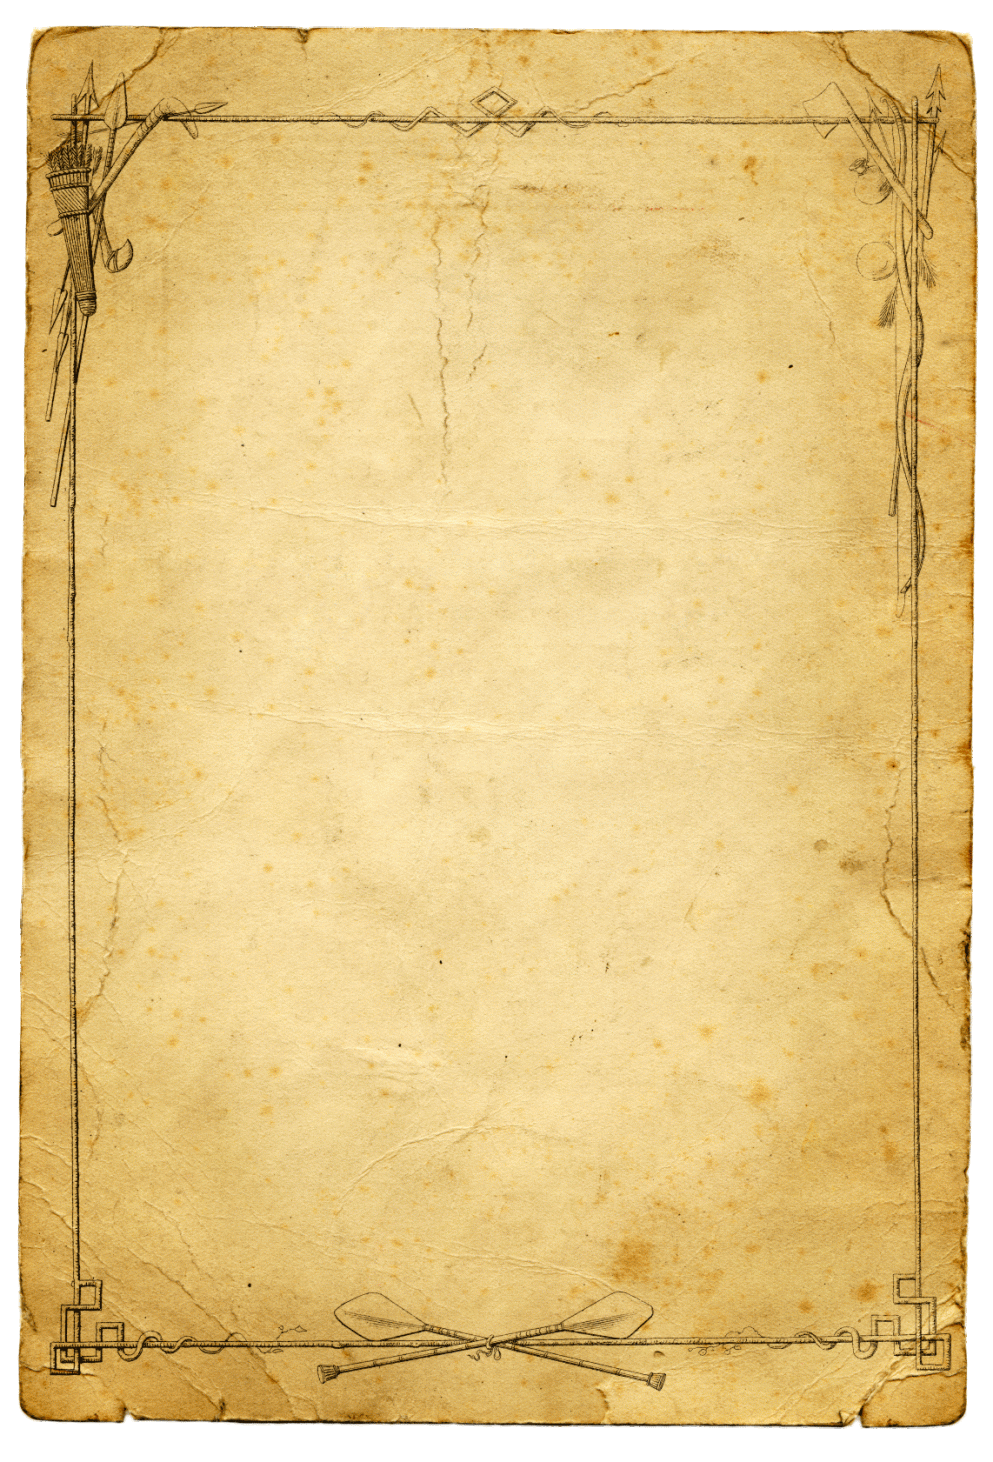
\includegraphics[
        width=\paperwidth,
        height=\paperheight
      ]{media/bkgd1}%
    };
  \end{tikzpicture}%
}

% Header
\fancyhead[LO,LE]{\color{headcolor}\rightmark}
\fancyhead[RE,RO]{\color{headcolor}\leftmark}

\renewcommand{\headrulewidth}{1.00pt}\color{rulecolor} % Rule under the header
\fancyfoot[C]{\textbf{\textsf{\thepage}}} % Bottom center footer
\renewcommand{\footrulewidth}{1.00pt}\color{rulecolor} % Rule under the footer
\pagestyle{fancy} % Use the custom headers and footers throughout the document


% Entries
% Entries
\newcommand{\entry}[6]{%
    \SetLetter{#1}%
    \vspace*{1mm}%
    \color{entrycolor}%
    \markboth{#1}{#1}%
    \textbf{#1}%
    \color{defcolor}%
    \ {#2}%
    \ \textit{#3}%
    \ $\bullet$\ {#4}%
    {#5}%
    {#6}%
}

% Redefining center
\let\oldcenter\center
\let\oldendcenter\endcenter
\renewenvironment{center}{\setlength\topsep{-5pt}\oldcenter}{\oldendcenter}


% Extracting entry first character
\newcommand{\FirstChar}[1]{%
    \StrLeft{#1}{1}[\firstletter]%
    \StrRight{#1}{1}[\lastletter]%
    \firstletter
}

\def \borderTextRight{\FirstChar{\rightmark}}
\def \borderTextLeft{\FirstChar{\leftmark}}

% \newcommand{\letter}[1]{\ifthenelse{\equal{#1}{A}}{\def \borderTextRight{OK}}{\def \borderTextRight{KO}}} % Under test

\AddToShipoutPictureFG{% from package eso-pic: put something to the background
	\ifthenelse{\isodd{\thepage}}{
		% ODD page: left bar
			\AtPageLowerLeft{% start the bar at the bottom right of the page
			\put(\LenToUnit{\dimexpr\paperwidth-1cm},0){% move it to the top right
				\color{bordercolor}
                    \rule{1cm}{\paperheight}%
			}%
             % Side letters
            \color{brickred}\put(575,820){\rotatebox{0}{\scalebox{2}{\borderTextRight}}}
            \color{lettercolor2}\put(569.5,805){\rotatebox{0}{\scalebox{2}{-----}}}
			            % \color{lettercolor3}\put(575,790){\rotatebox{0}{\scalebox{2}{A}}}
             % Alphabet latéral
                \LetterColor{A}\put(575,790){\scalebox{2}{A}}
                \LetterColor{B}\put(577,760){\scalebox{2}{B}}
                \LetterColor{C}\put(575,730){\scalebox{2}{C}}
                \LetterColor{D}\put(575,700){\scalebox{2}{D}}
                \LetterColor{E}\put(577,670){\scalebox{2}{E}}
                \LetterColor{F}\put(577,640){\scalebox{2}{F}}
                \LetterColor{G}\put(575,610){\scalebox{2}{G}}
                \LetterColor{H}\put(575,580){\scalebox{2}{H}}
                \LetterColor{I}\put(580,550){\scalebox{2}{I}}
                \LetterColor{J}\put(580,520){\scalebox{2}{J}}
                \LetterColor{K}\put(576,490){\scalebox{2}{K}}
                \LetterColor{L}\put(577,460){\scalebox{2}{L}}
                \LetterColor{M}\put(573,430){\scalebox{2}{M}}
                \LetterColor{N}\put(575,400){\scalebox{2}{N}}
                \LetterColor{O}\put(575,370){\scalebox{2}{O}}
                \LetterColor{P}\put(577,340){\scalebox{2}{P}}
                \LetterColor{Q}\put(575,310){\scalebox{2}{Q}}
                \LetterColor{R}\put(577,280){\scalebox{2}{R}}
                \LetterColor{S}\put(578,250){\scalebox{2}{S}}
                \LetterColor{T}\put(577,220){\scalebox{2}{T}}
                \LetterColor{U}\put(575,190){\scalebox{2}{U}}
                \LetterColor{V}\put(576,160){\scalebox{2}{V}}
                \LetterColor{W}\put(573,130){\scalebox{2}{W}}
                \LetterColor{X}\put(575,100){\scalebox{2}{X}}
                \LetterColor{Y}\put(575,70){\scalebox{2}{Y}}
                \LetterColor{Z}\put(575,40){\scalebox{2}{Z}}

            \color{lettercolor2}\put(569.5,25){\rotatebox{0}{\scalebox{2}{-----}}}
			\color{brickred}\put(575,10){\rotatebox{0}{\scalebox{2}{\borderTextLeft}}}
            
		}%
	
	}%
	{%
		% EVEN page: right bar
			\AtPageLowerLeft{% start the bar at the left bottom of the page
			\color{bordercolor}
                    \rule{1cm}{\paperheight}%

            % Side letters
            \color{brickred}\put(-15,820){\rotatebox{0}{\scalebox{2}{\borderTextRight}}}
	    	\color{lettercolor2}\put(-15.5,805){\rotatebox{0}{\scalebox{2}{-----}}}
			 % Alphabet latéral
                \LetterColor{A}\put(-15,790){\scalebox{2}{A}}
                \LetterColor{B}\put(-15,760){\scalebox{2}{B}}
                \LetterColor{C}\put(-15,730){\scalebox{2}{C}}
                \LetterColor{D}\put(-15,700){\scalebox{2}{D}}
                \LetterColor{E}\put(-15,670){\scalebox{2}{E}}
                \LetterColor{F}\put(-15,640){\scalebox{2}{F}}
                \LetterColor{G}\put(-15,610){\scalebox{2}{G}}
                \LetterColor{H}\put(-15,580){\scalebox{2}{H}}
                \LetterColor{I}\put(-15,550){\scalebox{2}{I}}
                \LetterColor{J}\put(-15,520){\scalebox{2}{J}}
                \LetterColor{K}\put(-15,490){\scalebox{2}{K}}
                \LetterColor{L}\put(-15,460){\scalebox{2}{L}}
                \LetterColor{M}\put(-15,430){\scalebox{2}{M}}
                \LetterColor{N}\put(-15,400){\scalebox{2}{N}}
                \LetterColor{O}\put(-15,370){\scalebox{2}{O}}
                \LetterColor{P}\put(-15,340){\scalebox{2}{P}}
                \LetterColor{Q}\put(-15,310){\scalebox{2}{Q}}
                \LetterColor{R}\put(-15,280){\scalebox{2}{R}}
                \LetterColor{S}\put(-15,250){\scalebox{2}{S}}
                \LetterColor{T}\put(-15,220){\scalebox{2}{T}}
                \LetterColor{U}\put(-15,190){\scalebox{2}{U}}
                \LetterColor{V}\put(-15,160){\scalebox{2}{V}}
                \LetterColor{W}\put(-15,130){\scalebox{2}{W}}
                \LetterColor{X}\put(-15,100){\scalebox{2}{X}}
                \LetterColor{Y}\put(-15,70){\scalebox{2}{Y}}
                \LetterColor{Z}\put(-15,40){\scalebox{2}{Z}}

            \color{lettercolor2}\put(-15.5,25){\rotatebox{0}{\scalebox{2}{-----}}}
            \color{brickred}\put(-15,10){\rotatebox{0}{\scalebox{2}{\borderTextLeft}}}

		}%
	
	}%
}



%----------------------------------------------------------------------------------------
\begin{document}

\begin{center}
    \Large{\lettrine[lines=1]{\color{titlecolor}D}{ictionnaire de Mots Valises}}\\
    \small{--- Alain Créhange ---}
\end{center}
\vspace{4mm}
\hrule height 1.0pt
\vspace{0mm}

\hrule height 0.5pt

\section*{U}
\refstepcounter{Uletter}\label{s:Uletter}

\hrule height 0.5pt

% ============================================================
% Généré automatiquement depuis : dico_data.csv
% Ne pas modifier manuellement.
% ============================================================

% Lettres présentes dans le dictionnaire
\letterAtrue
\letterBtrue
\letterCtrue
\letterDtrue
\letterEtrue
\letterFtrue
\letterGtrue
\letterHtrue
\letterItrue
\letterJtrue
\letterLtrue
\letterMtrue
\letterNtrue
\letterOtrue
\letterPtrue
\letterQtrue
\letterRtrue
\letterStrue
\letterTtrue
\letterVtrue

% Entrées du dictionnaire

\entry{à dessein}{}{}{Intentionnellement.}{}{CNRTL / Académie / analyse contextuelle}

\entry{à la fleur de l’âge}{}{}{À l’époque de la jeunesse, dans la période de pleine vigueur.}{Un bon petit diable à la fleur de l'âge, La jambe légère et l'œil polisson}{CNRTL / Académie / analyse contextuelle}

\entry{à la hussarde}{}{}{Brutalement, sans précaution ni délicatesse.}{}{CNRTL / Académie / analyse contextuelle}

\entry{à la va-comme-je-te-pousse}{}{}{Sans méthode, de façon improvisée et désordonnée.}{}{CNRTL / Académie / analyse contextuelle}

\entry{à l’emporte-pièce}{}{}{De façon brutale, tranchée ou sans nuance.}{}{CNRTL / Académie / analyse contextuelle}

\entry{à tout berzingue}{}{}{Très vite.}{}{CNRTL / Académie / analyse contextuelle}

\entry{à vau-l’eau}{}{}{En se dégradant, sans direction ni contrôle.}{}{CNRTL / Académie / analyse contextuelle}

\entry{affliction}{}{}{À vérifier dans un dictionnaire lexicographique.}{Disons que dans son affliction, Il trouve des compensations.}{CNRTL/TLFi ou Dictionnaire de l’Académie française}

\entry{aïeux}{}{}{À vérifier dans un dictionnaire lexicographique.}{Je serais honteux de mon sang, Des aïeux de qui je descends}{CNRTL/TLFi ou Dictionnaire de l’Académie française}

\entry{alangui}{}{}{À vérifier dans un dictionnaire lexicographique.}{Peu de chances qu'on voie mes belles odalisques, Déposer en grand deuil au pied de l'obélisque, Quelques gerbes de fleurs. Tout au plus gentiment diront-elles : « Peuchère, Le vieux Priape est mort », et, la cuisse légère, Le regard alangui,}{CNRTL/TLFi ou Dictionnaire de l’Académie française}

\entry{ambages}{}{}{À vérifier dans un dictionnaire lexicographique.}{Sans ambages, Dans les pages, Du missel,}{CNRTL/TLFi ou Dictionnaire de l’Académie française}

\entry{argousins}{}{}{À vérifier dans un dictionnaire lexicographique.}{Qu'il avait un petit cousin, au gué, au gué, Haut placé chez les argousins, au gué, au gué}{CNRTL/TLFi ou Dictionnaire de l’Académie française}

\entry{au diable Vauvert}{}{}{Très loin, dans un endroit éloigné.}{Emportent les trépassés jusqu'au diable vauvert}{CNRTL / Académie / analyse contextuelle}

\entry{aubade}{}{nom}{Musique ou chant donné au petit matin, traditionnellement sous les fenêtres de quelqu’un.}{J'ai graissé la patte au berger, Pour lui faire jouer une aubade.}{CNRTL/TLFi ou Dictionnaire de l’Académie française}

\entry{avecques}{}{}{À vérifier dans un dictionnaire lexicographique.}{D'avecques ma femme, J'ai foutu le camp}{CNRTL/TLFi ou Dictionnaire de l’Académie française}

\entry{avoir le cœur en fête}{}{}{Être très heureux.}{}{CNRTL / Académie / analyse contextuelle}

\entry{avoir les crocs}{}{}{Avoir très faim.}{}{CNRTL / Académie / analyse contextuelle}

\entry{avoir les yeux de Chimène}{}{}{Regarder quelqu’un avec amour ou admiration.}{}{CNRTL / Académie / analyse contextuelle}

\entry{avoir l’âme en peine}{}{}{Être triste, tourmenté ou malheureux.}{}{CNRTL / Académie / analyse contextuelle}

\entry{avoir maille à partir}{}{}{Avoir un différend, une querelle avec quelqu’un.}{}{CNRTL / Académie / analyse contextuelle}

\entry{avoir pignon sur rue}{}{}{Être bien établi, connu et respectable.}{}{CNRTL / Académie / analyse contextuelle}

\entry{avoir une âme en peine}{}{}{Être profondément triste ou affligé.}{}{CNRTL / Académie / analyse contextuelle}

\entry{battre sa coulpe}{}{}{Reconnaître sa faute, s’en accuser.}{}{CNRTL / Académie / analyse contextuelle}

\entry{bedeau}{}{nom}{Laïc chargé de certaines fonctions matérielles dans une église.}{L'maître d'école et ses potaches, le maire, le bedeau, le bougnat, négligeaient carrément leur tâche pour voir ça}{CNRTL/TLFi ou Dictionnaire de l’Académie française}

\entry{bélître}{}{}{À vérifier dans un dictionnaire lexicographique.}{On murmure in petto : « C'est un vrai Nicodème, Un balourd, un bélître, un bel âne bâté. »}{CNRTL/TLFi ou Dictionnaire de l’Académie française}

\entry{béotien}{}{nom/adj.}{Personne ignorante ou peu cultivée dans un domaine; à l’origine, habitant de Béotie.}{Hélas un béotien à la place du sien, lui proposa son blase}{CNRTL/TLFi ou Dictionnaire de l’Académie française}

\entry{bibine}{}{nom}{Bière, généralement bon marché, dans un emploi populaire.}{L'éponge trempée dans Dieu sait quelle bibine,}{CNRTL/TLFi ou Dictionnaire de l’Académie française}

\entry{bigot}{}{nom/adj.}{Personne attachée de manière étroite et excessive aux pratiques religieuses.}{J'ai perdu la tramontane, En perdant Margot, Qui épousa, contre son âme, Un triste bigot...}{CNRTL/TLFi ou Dictionnaire de l’Académie française}

\entry{billevesées}{}{}{À vérifier dans un dictionnaire lexicographique.}{Et les billevesées de tous les répertoires, Et les morts pour que naisse un avenir plus beau,}{CNRTL/TLFi ou Dictionnaire de l’Académie française}

\entry{bon gré mal gré}{}{}{Que cela plaise ou non.}{}{CNRTL / Académie / analyse contextuelle}

\entry{bordel}{}{}{À vérifier dans un dictionnaire lexicographique.}{Sitôt privée de ma tutelle, Ma pauvre amie, Courut essuyer du bordel, Les infamies}{CNRTL/TLFi ou Dictionnaire de l’Académie française}

\entry{bougnat}{}{nom}{Marchand de charbon et, traditionnellement, débitant de boissons d’origine auvergnate.}{L'maître d'école et ses potaches, le maire, le bedeau, le bougnat, négligeaient carrément leur tâche pour voir ça}{CNRTL/TLFi ou Dictionnaire de l’Académie française}

\entry{bourrelé}{}{adj.}{Qui est tourmenté ou accablé par un sentiment, notamment le remords.}{Le criminel saisi d'un zèle expiatoire, Qui bat sa coulpe bourrelé par le remords,}{CNRTL/TLFi ou Dictionnaire de l’Académie française}

\entry{braire}{}{verbe}{Crier, en parlant de l’âne; par extension, crier d’une manière désagréable.}{Elle eut beau pousser des sanglots, Braire à tue-tête, Comme je n'étais qu'un salaud, J'me fis honnête}{CNRTL/TLFi ou Dictionnaire de l’Académie française}

\entry{branque}{}{}{À vérifier dans un dictionnaire lexicographique.}{Qu'ils aient comme ce branque compté la musique pour moins que zéro}{CNRTL/TLFi ou Dictionnaire de l’Académie française}

\entry{brummel}{}{}{À vérifier dans un dictionnaire lexicographique.}{Tous les Brummel, les dandys, les gandins, il les considérait avec dédain}{CNRTL/TLFi ou Dictionnaire de l’Académie française}

\entry{bucolique}{}{}{À vérifier dans un dictionnaire lexicographique.}{Une adorable bucolique, Il est mélancolique}{CNRTL/TLFi ou Dictionnaire de l’Académie française}

\entry{callipyge}{}{adj.}{Qui a de belles fesses, bien proportionnées.}{VENUS CALLIPYGE}{CNRTL/TLFi ou Dictionnaire de l’Académie française}

\entry{calotins}{}{}{À vérifier dans un dictionnaire lexicographique.}{Ils ne savent pas ce qu'ils perdent, Tous ces fichus calotins, Sans le latin, sans le latin, La messe nous emmerde}{CNRTL/TLFi ou Dictionnaire de l’Académie française}

\entry{camarde}{}{}{À vérifier dans un dictionnaire lexicographique.}{Et Dieu fit signe à la camarde, De l'expédier rue Froidevaux...}{CNRTL/TLFi ou Dictionnaire de l’Académie française}

\entry{chaumine}{}{}{À vérifier dans un dictionnaire lexicographique.}{Vers son clocher, sa chaumine, Ses parents et sa promise}{CNRTL/TLFi ou Dictionnaire de l’Académie française}

\entry{chenue}{}{}{À vérifier dans un dictionnaire lexicographique.}{Il avait la tête chenue, Et le cœur ingénu}{CNRTL/TLFi ou Dictionnaire de l’Académie française}

\entry{chevet}{}{}{À vérifier dans un dictionnaire lexicographique.}{Ne vous étonnez pas, ma chère, Si vous trouvez, Les vers de jadis et naguère, A mon chevet.}{CNRTL/TLFi ou Dictionnaire de l’Académie française}

\entry{coi}{}{adj.}{Silencieux, sans parler; immobile et muet.}{Qu'je m'démène ou qu'je reste coi, Je passe pour un je-ne-sais-quoi !}{CNRTL/TLFi ou Dictionnaire de l’Académie française}

\entry{complainte}{}{}{À vérifier dans un dictionnaire lexicographique.}{Dieu fasse que ma complainte aille, tambour battant, Lui parler de la pluie, lui parler du gros temps}{CNRTL/TLFi ou Dictionnaire de l’Académie française}

\entry{cornegidouilles}{}{}{À vérifier dans un dictionnaire lexicographique.}{Tous les morbleus, tous les ventrebleus, Les sacrebleus et les cornegidouilles}{CNRTL/TLFi ou Dictionnaire de l’Académie française}

\entry{cornette}{}{}{À vérifier dans un dictionnaire lexicographique.}{Tous les cœurs se rallient à sa blanche cornette, Si le chrétien succombe à son charme insidieux,}{CNRTL/TLFi ou Dictionnaire de l’Académie française}

\entry{cotart}{}{}{À vérifier dans un dictionnaire lexicographique.}{L'âme du bon feu maistre Jehan Cotart, se réincarnait chez ce vieux fêtard.}{CNRTL/TLFi ou Dictionnaire de l’Académie française}

\entry{cotillon}{}{nom}{Jupe de femme, notamment dans un emploi ancien; danse populaire à l’origine.}{Quand il se fit tendre, elle lui dit : « J'présage, Qu'c'est pas dans les plis de mon cotillon}{CNRTL/TLFi ou Dictionnaire de l’Académie française}

\entry{couillonnades}{}{}{À vérifier dans un dictionnaire lexicographique.}{Soit dit sans couillonnades avait le nom d'un ad-jectif démonstratif}{CNRTL/TLFi ou Dictionnaire de l’Académie française}

\entry{coulpe}{}{nom}{Faute ou culpabilité, surtout dans « battre sa coulpe ».}{Le criminel saisi d'un zèle expiatoire, Qui bat sa coulpe bourrelé par le remords,}{CNRTL/TLFi ou Dictionnaire de l’Académie française}

\entry{cousette}{}{}{À vérifier dans un dictionnaire lexicographique.}{Qui brode, divine cousette, des arcs-en-ciel à nos chaussettes ?}{CNRTL/TLFi ou Dictionnaire de l’Académie française}

\entry{croquantes}{}{}{À vérifier dans un dictionnaire lexicographique.}{Toi qui m'as donné du feu quand, Les croquantes et les croquants}{CNRTL/TLFi ou Dictionnaire de l’Académie française}

\entry{croquants}{}{}{À vérifier dans un dictionnaire lexicographique.}{Toi qui m'as donné du feu quand, Les croquantes et les croquants}{CNRTL/TLFi ou Dictionnaire de l’Académie française}

\entry{croquignol}{}{adj./nom}{Ridicule, grotesque; personne ou situation comique par son aspect.}{Et donnèrent je vous l'assure, Un spectacle assez croquignol.}{CNRTL/TLFi ou Dictionnaire de l’Académie française}

\entry{crottés}{}{}{À vérifier dans un dictionnaire lexicographique.}{Les sabots d'Hélène, étaient tout crottés,}{CNRTL/TLFi ou Dictionnaire de l’Académie française}

\entry{crottin}{}{}{À vérifier dans un dictionnaire lexicographique.}{D'voir leurs héritiers marrons marcher dans le crottin}{CNRTL/TLFi ou Dictionnaire de l’Académie française}

\entry{danaïdes}{}{}{À vérifier dans un dictionnaire lexicographique.}{C'est le tonneau des Danaïdes changé en femme, Les joies charnelles m'emmerdent. \{2x\}}{CNRTL/TLFi ou Dictionnaire de l’Académie française}

\entry{dandys}{}{}{À vérifier dans un dictionnaire lexicographique.}{Tous les Brummel, les dandys, les gandins, il les considérait avec dédain}{CNRTL/TLFi ou Dictionnaire de l’Académie française}

\entry{de concert}{}{}{En accord ou ensemble avec d’autres.}{}{CNRTL / Académie / analyse contextuelle}

\entry{de conserve}{}{}{Ensemble, en commun; souvent à propos de personnes ou de navires.}{}{CNRTL / Académie / analyse contextuelle}

\entry{de haute lutte}{}{}{Après une lutte difficile et acharnée.}{}{CNRTL / Académie / analyse contextuelle}

\entry{délectable}{}{adj.}{Qui procure un grand plaisir, notamment au goût ou à l’esprit.}{La suite serait délectable, Malheureusement je ne peux,}{CNRTL/TLFi ou Dictionnaire de l’Académie française}

\entry{dès potron-minet}{}{}{Très tôt le matin, à l’aube.}{}{CNRTL / Académie / analyse contextuelle}

\entry{désempoissonnée}{}{}{À vérifier dans un dictionnaire lexicographique.}{Le crêpe à la queue sans doute, L'escorteront chagrinés, Laissant la rivière toute, Vide, désempoissonnée.}{CNRTL/TLFi ou Dictionnaire de l’Académie française}

\entry{donzelle}{}{nom}{Jeune fille ou femme, terme ancien ou plaisant.}{Me sentant rempli de pitié, Pour la donzelle, J'lui enseignai, de son métier, Les p'tites ficelles}{CNRTL/TLFi ou Dictionnaire de l’Académie française}

\entry{émule}{}{}{À vérifier dans un dictionnaire lexicographique.}{Quand on ne le veut point, un émule de Socrate,}{CNRTL/TLFi ou Dictionnaire de l’Académie française}

\entry{en filigrane}{}{}{De façon discrète mais perceptible en arrière-plan.}{}{CNRTL / Académie / analyse contextuelle}

\entry{en un tournemain}{}{}{Très rapidement et avec facilité.}{N'y allant pas par quatre chemins, J'estourbis en un tournemain}{CNRTL / Académie / analyse contextuelle}

\entry{engeance}{}{nom}{Race, espèce, descendance; souvent avec une nuance péjorative.}{Dès que la féminine engeance, sut que le singe était puceau}{CNRTL/TLFi ou Dictionnaire de l’Académie française}

\entry{espérance}{}{}{À vérifier dans un dictionnaire lexicographique.}{J'ai l'espérance qu'elle viendra, Faire sa niche entre mes bras, entre mes bras.}{CNRTL/TLFi ou Dictionnaire de l’Académie française}

\entry{être aux abois}{}{}{Être dans une situation désespérée, sans solution apparente.}{}{CNRTL / Académie / analyse contextuelle}

\entry{exutoires}{}{}{À vérifier dans un dictionnaire lexicographique.}{Le bagne, l'échafaud entre autres exutoires, Et l'efficacité de la peine de mort,}{CNRTL/TLFi ou Dictionnaire de l’Académie française}

\entry{fâcheux}{}{adj./nom}{Qui importune, ennuie ou contrarie; personne importune.}{Mais une attention profonde, Prouve que c'est chez les fâcheux, Qu'il préfère choisir les victimes de ses petits jeux}{CNRTL/TLFi ou Dictionnaire de l’Académie française}

\entry{faire bonne chère}{}{}{Bien manger; recevoir ou manger abondamment.}{}{CNRTL / Académie / analyse contextuelle}

\entry{faire des gorges chaudes}{}{}{Se moquer abondamment d’une personne ou d’un événement.}{}{CNRTL / Académie / analyse contextuelle}

\entry{faire fi de}{}{}{Ne pas tenir compte de; mépriser.}{}{CNRTL / Académie / analyse contextuelle}

\entry{faire florès}{}{}{Connaître un grand succès, être en vogue.}{}{CNRTL / Académie / analyse contextuelle}

\entry{faire la nique}{}{}{Se moquer de quelqu’un ou le défier par un geste de mépris.}{}{CNRTL / Académie / analyse contextuelle}

\entry{faire la pige au temps}{}{}{Rivaliser avec le temps, tenter de lui échapper ou de le tromper.}{}{CNRTL / Académie / analyse contextuelle}

\entry{faire long feu}{}{}{Échouer ou ne pas produire l’effet attendu; selon l’usage, durer plus longtemps que prévu.}{}{CNRTL / Académie / analyse contextuelle}

\entry{faire route}{}{}{Se diriger vers un lieu, voyager dans une direction donnée.}{}{CNRTL / Académie / analyse contextuelle}

\entry{faire un four}{}{}{Subir un échec, notamment pour un spectacle ou une entreprise.}{}{CNRTL / Académie / analyse contextuelle}

\entry{fretin}{}{nom}{Petit poisson; au figuré, personnes ou choses de peu d’importance.}{Mais s'il pêche, c'est pour rire, Et l'on peut être certain, Que jamais sa poêle à frire, Vit le plus menu fretin.}{CNRTL/TLFi ou Dictionnaire de l’Académie française}

\entry{froufrous}{}{}{À vérifier dans un dictionnaire lexicographique.}{La demeure que je préfère, C'est votre robe à froufrous}{CNRTL/TLFi ou Dictionnaire de l’Académie française}

\entry{gambades}{}{}{À vérifier dans un dictionnaire lexicographique.}{Lors ma mie, sans croire au danger, Faisons mille et une gambades,}{CNRTL/TLFi ou Dictionnaire de l’Académie française}

\entry{gandins}{}{}{À vérifier dans un dictionnaire lexicographique.}{Tous les Brummel, les dandys, les gandins, il les considérait avec dédain}{CNRTL/TLFi ou Dictionnaire de l’Académie française}

\entry{gargotière}{}{nom}{Femme qui tient une gargote.}{Madame ma gargotière, Comme je lui dois trop de sous}{CNRTL/TLFi ou Dictionnaire de l’Académie française}

\entry{gastibelza}{}{}{À vérifier dans un dictionnaire lexicographique.}{GASTIBELZA "L'HOMME A LA CARABINE"}{CNRTL/TLFi ou Dictionnaire de l’Académie française}

\entry{gendarmicides}{}{}{À vérifier dans un dictionnaire lexicographique.}{Des mégères gendarmicides, En criant: « Hip, hip, hip, hourra ! »}{CNRTL/TLFi ou Dictionnaire de l’Académie française}

\entry{gentilhommière}{}{nom}{Petite demeure de campagne appartenant à un gentilhomme.}{Je changerais ma chaumière, Pour une gentilhommière}{CNRTL/TLFi ou Dictionnaire de l’Académie française}

\entry{gentilhommières}{}{}{À vérifier dans un dictionnaire lexicographique.}{Où le septième ciel, ma plus chère ballade, Ma plus douce grimpette et plus tendre escalade, Sera trop haut pour moi. Il n'y aura pas de pleurs dans les gentilhommières, Ni de grincements de fesses dans les chaumières, Faut pas que je me leurre.}{CNRTL/TLFi ou Dictionnaire de l’Académie française}

\entry{gibus}{}{}{À vérifier dans un dictionnaire lexicographique.}{J'ai des velléités d'arpenter les trottoir(e)s, Avec cette devise écrite à mon gibus :}{CNRTL/TLFi ou Dictionnaire de l’Académie française}

\entry{gnons}{}{}{À vérifier dans un dictionnaire lexicographique.}{Jugeant enfin que leurs victimes, Avaient eu leur content de gnons}{CNRTL/TLFi ou Dictionnaire de l’Académie française}

\entry{goton}{}{nom}{Femme ou fille de condition modeste; nom populaire et vieilli.}{Et plus belle d'une goton. Dieu, s'il existe, il exagère,}{CNRTL/TLFi ou Dictionnaire de l’Académie française}

\entry{goualante}{}{nom}{Chanson populaire, souvent d’argot ou de rue.}{Poussant une autre goualante y'aurait à ma place un autre cabot}{CNRTL/TLFi ou Dictionnaire de l’Académie française}

\entry{gougoutte}{}{}{À vérifier dans un dictionnaire lexicographique.}{Quand Margot dégrafait son corsage, pour donner la gougoutte à son chat}{CNRTL/TLFi ou Dictionnaire de l’Académie française}

\entry{goupillon}{}{}{À vérifier dans un dictionnaire lexicographique.}{Et l'on courut à toutes jambes, Quérir un goupillon mais}{CNRTL/TLFi ou Dictionnaire de l’Académie française}

\entry{gourgandines}{}{}{À vérifier dans un dictionnaire lexicographique.}{Mais s'il attrape une ondine, L'une de ces gourgandines, Femme mi-chair mi-poisson, Le polisson}{CNRTL/TLFi ou Dictionnaire de l’Académie française}

\entry{grégeois}{}{}{À vérifier dans un dictionnaire lexicographique.}{Et l'Espagne flambait dans un grand feu grégeois. Je chantais, et j'étais pas le seul « Y a d'la joie ».}{CNRTL/TLFi ou Dictionnaire de l’Académie française}

\entry{guilleret}{}{adj.}{Gai, enjoué, de bonne humeur.}{Laisse-moi tenir ton jupon, Courons guilleret, guillerette,}{CNRTL/TLFi ou Dictionnaire de l’Académie française}

\entry{guillerette}{}{}{À vérifier dans un dictionnaire lexicographique.}{Laisse-moi tenir ton jupon, Courons guilleret, guillerette,}{CNRTL/TLFi ou Dictionnaire de l’Académie française}

\entry{halieutique}{}{adj.}{Relatif à la pêche, notamment à la pêche maritime.}{On dirait un fanatique, De la cause halieutique, Avec sa belle canne et, Son moulinet.}{CNRTL/TLFi ou Dictionnaire de l’Académie française}

\entry{hottentots}{}{}{À vérifier dans un dictionnaire lexicographique.}{Callipyge à prétendre jouer les Vénus chez les Hottentots}{CNRTL/TLFi ou Dictionnaire de l’Académie française}

\entry{infamie}{}{}{À vérifier dans un dictionnaire lexicographique.}{Trouverais-je les noms, trouverais-je les mots, Pour noter d'infamie cet enfant de chameau}{CNRTL/TLFi ou Dictionnaire de l’Académie française}

\entry{ingénu}{}{}{À vérifier dans un dictionnaire lexicographique.}{Faut s'lever de bon matin pour voir un ingénu, Qui n't'ait pas connue,}{CNRTL/TLFi ou Dictionnaire de l’Académie française}

\entry{jarnibleus}{}{}{À vérifier dans un dictionnaire lexicographique.}{Ainsi, parbleu, que les jarnibleus, Et les palsambleus}{CNRTL/TLFi ou Dictionnaire de l’Académie française}

\entry{jarnicotons}{}{interj.}{Juron fantaisiste, variation populaire de jurons anciens.}{Sans oublier les jarnicotons, Les scrogneugneus et les bigres et les bougres}{CNRTL/TLFi ou Dictionnaire de l’Académie française}

\entry{jobastre}{}{nom/adj.}{Personne extravagante, maladroite ou stupide; terme populaire.}{Si le sieur Z était un jobastre sans grade, Il laisserait en paix ses pauvres camarades.}{CNRTL/TLFi ou Dictionnaire de l’Académie française}

\entry{jouer des fesses}{}{}{Bouger ou utiliser ses fesses de façon suggestive; dans le texte, se mouvoir de manière sexuelle.}{Car, dans l'art de faire le trottoir, Je le confesse, Le difficile est d'bien savoir, Jouer des fesses}{CNRTL / Académie / analyse contextuelle}

\entry{jouvenceau}{}{nom}{Jeune homme, garçon encore très jeune.}{Depuis que je commence à faire de vieux os, Avide de conseils, souvent un jouvenceau}{CNRTL/TLFi ou Dictionnaire de l’Académie française}

\entry{lâcher la bride à son émoi}{}{}{Laisser libre cours à son émotion.}{}{CNRTL / Académie / analyse contextuelle}

\entry{lacune}{}{}{À vérifier dans un dictionnaire lexicographique.}{C'est : « enculé ». Lacune comblée.}{CNRTL/TLFi ou Dictionnaire de l’Académie française}

\entry{languedo}{}{}{À vérifier dans un dictionnaire lexicographique.}{Dans les années quarante où je débarquais de mon Languedo}{CNRTL/TLFi ou Dictionnaire de l’Académie française}

\entry{lapidaire}{}{adj.}{Très concis, réduit à l’essentiel; relatif aussi à la taille ou au commerce des pierres.}{Ils gravent sur mon mur en style lapidaire : « Ici loge un vieux bouc qui n'a plus d'érections ! » Ils sont prématurés, tous ces cris de victoire, Ô vous qui me plantez la corne dans le dos,}{CNRTL/TLFi ou Dictionnaire de l’Académie française}

\entry{licou}{}{nom}{Licol, dispositif de cuir ou de corde placé sur la tête d’un animal.}{Menait César, empereur d'Allemagne, Par le licou... -Le vent qui vient à travers la montagne Me rendra fou.}{CNRTL/TLFi ou Dictionnaire de l’Académie française}

\entry{lorgner}{}{}{À vérifier dans un dictionnaire lexicographique.}{A l'heure du repas, mes rivaux détestables, Ont encor ce toupet de lorgner ma portion}{CNRTL/TLFi ou Dictionnaire de l’Académie française}

\entry{lourdauds}{}{}{À vérifier dans un dictionnaire lexicographique.}{Une autre fourre avec rudesse, Le crâne d'un de ses lourdauds}{CNRTL/TLFi ou Dictionnaire de l’Académie française}

\entry{lurette}{}{}{À vérifier dans un dictionnaire lexicographique.}{Voici belle lurette, en fut le vrai premier.}{CNRTL/TLFi ou Dictionnaire de l’Académie française}

\entry{macchabées}{}{}{À vérifier dans un dictionnaire lexicographique.}{Moi, j'bichais car je les adore, Sous la forme de macchabées}{CNRTL/TLFi ou Dictionnaire de l’Académie française}

\entry{madone}{}{nom}{La Vierge Marie représentée dans l’art; par extension, représentation de la Vierge.}{J'lui ai dit: « De la Madone, Tu es le portrait ! » Le Bon Dieu me le pardonne, C'était un peu vrai...}{CNRTL/TLFi ou Dictionnaire de l’Académie française}

\entry{maraud}{}{nom/adj.}{Personne grossière, malhonnête ou méprisable; parfois terme d’injure.}{Si, par hasard, Sur l'Pont des Arts, Tu croises le vent, le vent maraud, Prudent, prends garde à ton chapeau}{CNRTL/TLFi ou Dictionnaire de l’Académie française}

\entry{maritornes}{}{nom}{Femmes grossières ou peu séduisantes; par référence au personnage de Maritorne dans Don Quichotte.}{Un truc, un moyen plausible, De fuir un peu son chez-soi, Où sévit la plus nuisible, Des maritornes qui soient.}{CNRTL/TLFi ou Dictionnaire de l’Académie française}

\entry{matamore}{}{nom}{Fanfaron, vantard qui se donne des airs de héros.}{Mais il est général, va-t-en-guerre, matamore. Dès qu'il s'en mêle, on compte les morts.}{CNRTL/TLFi ou Dictionnaire de l’Académie française}

\entry{matines}{}{}{À vérifier dans un dictionnaire lexicographique.}{Ding ding dong, les matines sonnent, En l'honneur de notre bonheur,}{CNRTL/TLFi ou Dictionnaire de l’Académie française}

\entry{maugrabine}{}{nom}{Femme originaire du Maghreb ou, dans un emploi ancien, de l’Afrique du Nord.}{« Quelqu'un de vous a-t-il connu Sabine, Ma señora ? Sa mère était la vieille maugrabine D'Antequera,}{CNRTL/TLFi ou Dictionnaire de l’Académie française}

\entry{mégères}{}{}{À vérifier dans un dictionnaire lexicographique.}{Des mégères gendarmicides, En criant: « Hip, hip, hip, hourra ! »}{CNRTL/TLFi ou Dictionnaire de l’Académie française}

\entry{mener par le bout du cœur}{}{}{Exercer sur quelqu’un une forte emprise affective.}{}{CNRTL / Académie / analyse contextuelle}

\entry{méritoire}{}{}{À vérifier dans un dictionnaire lexicographique.}{« Le meilleur d'entre nous et le plus méritoire », « Un saint homme, un cœur d'or, un bel et noble esprit »}{CNRTL/TLFi ou Dictionnaire de l’Académie française}

\entry{métempsycose}{}{nom}{Passage de l’âme d’un corps dans un autre après la mort.}{Métamorphose inouïe, métempsycose infâme, Les joies charnelles me perdent,}{CNRTL/TLFi ou Dictionnaire de l’Académie française}

\entry{mettre à feu et à sang}{}{}{Dévaster, ravager; causer de grands dégâts.}{}{CNRTL / Académie / analyse contextuelle}

\entry{morbleu}{}{interj.}{Juronnement ancien, euphémisme de « mort de Dieu ».}{Souvenir de la cane, De Jeanne, Morbleu}{CNRTL/TLFi ou Dictionnaire de l’Académie française}

\entry{morpionibus}{}{locution}{Formule latinisante et fantaisiste utilisée comme jeu verbal autour du mot « morpion ».}{Et quand il y alla de ses De Profondis, L'enfant de cœur répliqua pas morpionibus}{CNRTL/TLFi ou Dictionnaire de l’Académie française}

\entry{naturalibus}{}{locution}{Nu, sans vêtements, dans l’expression « in naturalibus ».}{Qui'est-ce qui veut m'laisser faire, in naturalibus, Un p'tit peu d'alpinisme sur son mont de Vénus}{CNRTL/TLFi ou Dictionnaire de l’Académie française}

\entry{navrance}{}{nom}{État de grande tristesse, de désolation ou de découragement.}{On lirait quelle navrance mon blase inconnu dans un ex-voto}{CNRTL/TLFi ou Dictionnaire de l’Académie française}

\entry{nectar}{}{}{À vérifier dans un dictionnaire lexicographique.}{Va boire à Passy, Le nectar d'ici, Te dépasse.}{CNRTL/TLFi ou Dictionnaire de l’Académie française}

\entry{nonnettes}{}{}{À vérifier dans un dictionnaire lexicographique.}{De nonnettes, De cornettes, En sabbat,}{CNRTL/TLFi ou Dictionnaire de l’Académie française}

\entry{odalisques}{}{}{À vérifier dans un dictionnaire lexicographique.}{}{}

\entry{onaniste}{}{}{À vérifier dans un dictionnaire lexicographique.}{La moitié des messieurs brûle d'être onaniste,}{CNRTL/TLFi ou Dictionnaire de l’Académie française}

\entry{oraisons}{}{}{À vérifier dans un dictionnaire lexicographique.}{Sur les tombeaux les oraisons déclamatoires, Les : « C'était un bon fils, bon père, bon mari »,}{CNRTL/TLFi ou Dictionnaire de l’Académie française}

\entry{oriflamme}{}{nom}{Bannière ou étendard, notamment historique; au figuré, symbole ou signe de ralliement.}{Il conquit un oriflamme teuton. Cet acte lui valut le grand cordon.}{CNRTL/TLFi ou Dictionnaire de l’Académie française}

\entry{ostrogoth}{}{}{À vérifier dans un dictionnaire lexicographique.}{Au premier ostrogoth venu, Les croquants, ça tombe des nues}{CNRTL/TLFi ou Dictionnaire de l’Académie française}

\entry{palsambleus}{}{}{À vérifier dans un dictionnaire lexicographique.}{Ainsi, parbleu, que les jarnibleus, Et les palsambleus}{CNRTL/TLFi ou Dictionnaire de l’Académie française}

\entry{pandores}{}{}{À vérifier dans un dictionnaire lexicographique.}{En voyant ces braves pandores, Être à deux doigts de succomber}{CNRTL/TLFi ou Dictionnaire de l’Académie française}

\entry{pâquerette}{}{}{À vérifier dans un dictionnaire lexicographique.}{Indiscrète, Pâquerette, D'où vient-elle ?}{CNRTL/TLFi ou Dictionnaire de l’Académie française}

\entry{pardi}{}{interj.}{Forme populaire de « par Dieu », employée pour renforcer une affirmation.}{Je n'perdais pas au change, pardi}{CNRTL/TLFi ou Dictionnaire de l’Académie française}

\entry{pastourelle}{}{nom}{Petit poème ou chanson médiévale mettant en scène un berger ou une bergère; par extension, genre pastoral.}{Et là-dessus le Corydon, Le promis de la pastourelle,}{CNRTL/TLFi ou Dictionnaire de l’Académie française}

\entry{patibulaire}{}{adj.}{Qui a une apparence inquiétante, suspecte ou peu rassurante.}{Je serais mort, jambes en l'air, Sur la veuve patibulaire,}{CNRTL/TLFi ou Dictionnaire de l’Académie française}

\entry{pécore}{}{}{À vérifier dans un dictionnaire lexicographique.}{Fils de pécore et de minus, Ris par de la pauvre Vénus}{CNRTL/TLFi ou Dictionnaire de l’Académie française}

\entry{peloteur}{}{nom}{Personne qui cherche à caresser ou à toucher quelqu’un de manière importune.}{Grand peloteur de fesses convaincu, passé maître en l'art de la main au cul,}{CNRTL/TLFi ou Dictionnaire de l’Académie française}

\entry{pétaudière}{}{nom}{Lieu ou assemblée où règnent le désordre et la confusion.}{En mélangeant les genres, vous avez fait d'la terre, Ce qu'elle est : une pétaudière !}{CNRTL/TLFi ou Dictionnaire de l’Académie française}

\entry{phallocrate}{}{}{À vérifier dans un dictionnaire lexicographique.}{Quand on veut les trousser, on est un phallocrate,}{CNRTL/TLFi ou Dictionnaire de l’Académie française}

\entry{pimpant}{}{adj.}{Joli, bien mis, élégant ou plein de vivacité.}{Et tout pimpant, tout satisfait, Prit la clef du champ de navets.}{CNRTL/TLFi ou Dictionnaire de l’Académie française}

\entry{pissotant}{}{}{À vérifier dans un dictionnaire lexicographique.}{Un soir d'intempérance, à son insu, il éteignit en pissotant dessus}{CNRTL/TLFi ou Dictionnaire de l’Académie française}

\entry{populo}{}{}{À vérifier dans un dictionnaire lexicographique.}{A qui fera-t-on croire que le bon populo, quand il chante quand même, est un parfait salaud ?}{CNRTL/TLFi ou Dictionnaire de l’Académie française}

\entry{pourceau}{}{}{À vérifier dans un dictionnaire lexicographique.}{Que le fameux cochon, le pourceau d'Epicure, Qui sommeillait en moi ne s'éveillera plus. Ils me croient interdit de séjour à Cythère, Et, par les nuits sans lune avec jubilation,}{CNRTL/TLFi ou Dictionnaire de l’Académie française}

\entry{prendre la mort comme elle vient}{}{}{Accepter la mort sans chercher à la maîtriser.}{Et jamais je ne parviens, A prendre la mort comme elle vient,}{CNRTL / Académie / analyse contextuelle}

\entry{preste}{}{adj.}{Rapide et agile dans ses mouvements.}{Le facteur d'ordinaire si preste pour voir ça ne distribuait plus les lettres que personne au reste n'aurait lues}{CNRTL/TLFi ou Dictionnaire de l’Académie française}

\entry{priape}{}{}{À vérifier dans un dictionnaire lexicographique.}{Peu de chances qu'on voie mes belles odalisques, Déposer en grand deuil au pied de l'obélisque, Quelques gerbes de fleurs. Tout au plus gentiment diront-elles : « Peuchère, Le vieux Priape est mort », et, la cuisse légère, Le regard alangui,}{CNRTL/TLFi ou Dictionnaire de l’Académie française}

\entry{probes}{}{}{À vérifier dans un dictionnaire lexicographique.}{Les jean-foutre et les gens probes, Médisent du vent furibond, Qui rebrousse les bois, détrousse les toits, retrousse les robes}{CNRTL/TLFi ou Dictionnaire de l’Académie française}

\entry{quadrumane}{}{nom/adj.}{Qui a quatre membres préhensiles; ancien terme appliqué notamment aux singes.}{Voyant que toutes se dérobe, Le quadrumane accéléra,}{CNRTL/TLFi ou Dictionnaire de l’Académie française}

\entry{quenouille}{}{nom}{Bâton servant à filer les fibres textiles; par extension, objet ayant une forme allongée.}{Comme il atteignait l'orée du village, Filant sa quenouille, il vit Cendrillon}{CNRTL/TLFi ou Dictionnaire de l’Académie française}

\entry{réquisitoire}{}{}{À vérifier dans un dictionnaire lexicographique.}{Fatigué de souffrir leur long réquisitoire}{CNRTL/TLFi ou Dictionnaire de l’Académie française}

\entry{retourner à ses oignons}{}{}{Revenir à ses propres affaires; se mêler de ce qui nous concerne.}{}{CNRTL / Académie / analyse contextuelle}

\entry{ritournelles}{}{}{À vérifier dans un dictionnaire lexicographique.}{Le feu de la ville éternelle est éternel. Si Dieu veut l'incendie, il veut les ritournelles.}{CNRTL/TLFi ou Dictionnaire de l’Académie française}

\entry{rogaton}{}{nom}{Objet sans valeur, petit reste ou écrit insignifiant; anciennement, reste de nourriture.}{Sans laisser même un rogaton, Tout il croque, tout il digère.}{CNRTL/TLFi ou Dictionnaire de l’Académie française}

\entry{sacrebleu}{}{}{À vérifier dans un dictionnaire lexicographique.}{Bande à part, sacrebleu ! c'est ma règle et j'y tiens. Dans les noms des partants on n'verra pas le mien.}{CNRTL/TLFi ou Dictionnaire de l’Académie française}

\entry{sacristain}{}{nom}{Personne chargée de la garde et de l’entretien d’une église et de ses objets liturgiques.}{On n'tortille pas son popotin, D'la même manière, Pour un droguiste, un sacristain, Un fonctionnaire}{CNRTL/TLFi ou Dictionnaire de l’Académie française}

\entry{sans ambages}{}{}{Directement, sans détour.}{Sans ambages, Dans les pages, Du missel,}{CNRTL / Académie / analyse contextuelle}

\entry{sans coup férir}{}{}{Sans rencontrer de résistance.}{}{CNRTL / Académie / analyse contextuelle}

\entry{sans vergogne}{}{}{Sans honte ni gêne.}{T'as couru sans vergogne, et pour une escalope, Te jeter dans le lit du boucher.}{CNRTL / Académie / analyse contextuelle}

\entry{sbires}{}{}{À vérifier dans un dictionnaire lexicographique.}{Deux sbires sont venus, avec leur noirs manteaux, entre la rue Didot et la rue de Vanves}{CNRTL/TLFi ou Dictionnaire de l’Académie française}

\entry{séguedille}{}{nom}{Danse et chant espagnols d’origine populaire, à rythme vif.}{Un pied pour la séguedille, un pied pour, La gaie tarentelle.}{CNRTL/TLFi ou Dictionnaire de l’Académie française}

\entry{sinécure}{}{}{À vérifier dans un dictionnaire lexicographique.}{Parc' que depuis tant d'années, C'était pas une sinécure}{CNRTL/TLFi ou Dictionnaire de l’Académie française}

\entry{subito}{}{}{À vérifier dans un dictionnaire lexicographique.}{La souris grise se fâche, et subito presto, entre la rue Didot et la rue de Vanves}{CNRTL/TLFi ou Dictionnaire de l’Académie française}

\entry{suffragettes}{}{}{À vérifier dans un dictionnaire lexicographique.}{A force d'être en butte au tir des suffragettes}{CNRTL/TLFi ou Dictionnaire de l’Académie française}

\entry{supplique}{}{}{À vérifier dans un dictionnaire lexicographique.}{05 - Supplique pour être enterré sur la plage de Sète\_sans\_accords}{CNRTL/TLFi ou Dictionnaire de l’Académie française}

\entry{tarabuste}{}{}{À vérifier dans un dictionnaire lexicographique.}{C'est très inconfortable et ça vous tarabuste,}{CNRTL/TLFi ou Dictionnaire de l’Académie française}

\entry{tendre la patte}{}{}{Demander ou recevoir de l’argent ou une aide; selon le contexte, solliciter une faveur.}{}{CNRTL / Académie / analyse contextuelle}

\entry{tenir la dragée haute}{}{}{Résister avec succès à quelqu’un, lui donner du fil à retordre.}{}{CNRTL / Académie / analyse contextuelle}

\entry{têtes chenues}{}{}{Têtes blanchies par l’âge; image traditionnelle de la vieillesse.}{Quand ils sont dev'nus des têtes chenues, des grisons}{CNRTL / Académie / analyse contextuelle}

\entry{teuton}{}{adj./nom}{Allemand, en emploi familier ou péjoratif, par référence aux anciens Teutons.}{Il conquit un oriflamme teuton. Cet acte lui valut le grand cordon.}{CNRTL/TLFi ou Dictionnaire de l’Académie française}

\entry{tout de go}{}{}{Directement, sans détour ni préparation.}{Le chat la prenant pour sa mère se mit à téter tout de go, émue Margot le laissa faire brave Margot}{CNRTL / Académie / analyse contextuelle}

\entry{tramontane}{}{nom}{Vent froid et sec venant du nord-ouest dans le Midi de la France; au figuré, idée de vent ou de perte de repères.}{J'ai perdu la tramontane En trouvant Margot, Princesse vêtue de laine, Déesse en sabots...}{CNRTL/TLFi ou Dictionnaire de l’Académie française}

\entry{transcendant}{}{}{À vérifier dans un dictionnaire lexicographique.}{Taisons-le, j'aurais bonne mine. Il me paraît plus transcendant}{CNRTL/TLFi ou Dictionnaire de l’Académie française}

\entry{transi}{}{}{À vérifier dans un dictionnaire lexicographique.}{Malheureux, poussiéreux, transi, Chante : « Ah ! ce qu'on s'emmerde ici » !}{CNRTL/TLFi ou Dictionnaire de l’Académie française}

\entry{valseur}{}{}{À vérifier dans un dictionnaire lexicographique.}{La louche au valseur; pas de ça Lisette ! La légion d'honneur ça pardonne pas.}{CNRTL/TLFi ou Dictionnaire de l’Académie française}

\entry{vauvert}{}{nom propre / locution}{Nom historique du Val-de-Green; présent dans l’expression « au diable Vauvert ».}{Emportent les trépassés jusqu'au diable vauvert}{CNRTL/TLFi ou Dictionnaire de l’Académie française}

\entry{ventrebleu}{}{}{À vérifier dans un dictionnaire lexicographique.}{Avec qui, ventrebleu, faut-il que je couche, Pour faire parler un peu la déesse aux cent bouches}{CNRTL/TLFi ou Dictionnaire de l’Académie française}

\entry{vêpres}{}{nom}{Office religieux célébré en fin d’après-midi ou le soir.}{La mignonne allait aux vêpres, Se mettre à genoux, Alors j'ai mordu ses lèvres, Pour savoir leur goût...}{CNRTL/TLFi ou Dictionnaire de l’Académie française}

\entry{vertudieux}{}{adj.}{Qui affecte ou manifeste une vertu morale ostentatoire.}{Tous les Bon Dieu, Tous les vertudieux, Tonnerre de Brest et saperlipopette}{CNRTL/TLFi ou Dictionnaire de l’Académie française}

\entry{viatique}{}{nom}{Sacrement ou secours spirituel donné à un mourant; au figuré, ressource emportée pour un voyage.}{Pour offrir à l'ancêtre, en signe d'affection, En guise de viatique, une ultime audition (bis)}{CNRTL/TLFi ou Dictionnaire de l’Académie française}

\entry{vicaire}{}{}{À vérifier dans un dictionnaire lexicographique.}{Avant même que le vicaire, Ait pu lâcher un cri}{CNRTL/TLFi ou Dictionnaire de l’Académie française}

\entry{vocables}{}{nom}{Mots, termes ou expressions considérés sous leur aspect lexical.}{Brillait par son absence un des pires vocables}{CNRTL/TLFi ou Dictionnaire de l’Académie française}

\entry{voir des deux yeux}{}{}{Constater directement, par opposition à croire sur parole.}{}{CNRTL / Académie / analyse contextuelle}

%\entry{bélître}{}{}{À vérifier dans un dictionnaire lexicographique.}{On murmure in petto : « C'est un vrai Nicodème, Un balourd, un bélître, un bel âne bâté. »}{CNRTL/TLFi ou Dictionnaire de l’Académie française}

	%------------------------------------------------
\end{document}
